% LaTeX template for Stat 4352.002: Mathematical Statistics
% University of Texas at Dallas, Spring 2026
% Yun Wei

\documentclass{article}
\usepackage{scribe} % specifies page and header format

% Useful packages

\RequirePackage{amsthm,amsmath,amsfonts,amssymb}
\RequirePackage{mathrsfs} % mathscr fonts
\RequirePackage{color}
\RequirePackage{enumitem}
\RequirePackage{mathtools}  % have the second line for subscript
\RequirePackage{verbatim} % to comment block
\RequirePackage{bm} % to change font to be both bold and ??it possible

% Theorem type environments

\theoremstyle{plain}
\newtheorem{thm}{Theorem}[section]
\newtheorem{lem}[thm]{Lemma}
\newtheorem{prop}[thm]{Proposition}
\newtheorem{cor}[thm]{Corollary}

\theoremstyle{definition}
\newtheorem{rem}[thm]{Remark}
\newtheorem{assump}[thm]{Assumption}
\newtheorem{prob}[thm]{Problem}
\newtheorem{exa}[thm]{Example}
\newtheorem{definition}[thm]{Definition}

\newcommand\numberthis{\addtocounter{equation}{1}\tag{\theequation}}

% Useful macros -- you can add your own

\newcommand{\sH}{{\mathcal H}}
\newcommand{\sX}{{\mathcal X}}
\newcommand{\sY}{{\mathcal Y}}
\newcommand{\hnhat}{\widehat{h}_n}

% frequently used symbols
\newcommand{\bbE}{\mathbb{E}} % use this for expectation
\newcommand{\bbR}{\mathbb{R}} % real numbers

% operators
\newcommand{\sign}{\mathop{\mathrm{sign}}}
\newcommand{\supp}{\mathop{\mathrm{supp}}} % support
\newcommand{\argmin}{\operatornamewithlimits{arg\ min}}
\newcommand{\argmax}{\operatornamewithlimits{arg\ max}}

% indicator function
\newcommand{\ind}[1]{\bm{1}_{\{#1\}}}

% grouping operators
\newcommand{\brac}[1]{\left[#1\right]}
\newcommand{\set}[1]{\left\{#1\right\}}
\newcommand{\abs}[1]{\left\lvert #1 \right\rvert}
\newcommand{\paren}[1]{\left(#1\right)}
\newcommand{\norm}[1]{\left\|#1\right\|}

\begin{document}

% Lecture header format:
%\lecture{**TOPIC-NUMBER**}{**TITLE**}{**LECTURER**}{**SCRIBE**}
\lecture{1}{Title}{Yun Wei}{Yun}

\noindent {\bf Disclaimer}: {\it These notes have not been subjected to
the usual scrutiny reserved for formal publications.  They may be
distributed outside this class only with the permission of the
Instructor.} %\vspace*{2mm}

\section{Introduction}

Some introductory remarks go here. This should be a brief paragraph that
sets the stage for what is to follow.  Connect to previous lectures if
possible.

\section{\LaTeX}

Firstly zip the files {\tt template.tex}, {\tt
scribe.sty},  {\tt example\_fig.png}  and {\tt lec001.tex}. Then in overleaf.com, select "new project", then "upload project" and then upload the zip files.  Then select {\tt template.tex} and then click "complie", and you generate this document. If you select {\tt lec001.tex} and then "complie", and you generate the pdf for lecture note 1.

%in the same directory, and then compile it in overleaf. 

%type
%\begin{verbatim}
%pdflatex template
%\end{verbatim}
%at the command prompt. Rerun the command if it complains about undefined
%labels or references.

You can find LaTeX tutorials on the Internet. %I have also uploaded a useful file of LaTeX symbols to CTools. 
You can also read the {\tt template.tex} and {\tt lec001.tex} to get a sense how it works. Ask me or your classmates or AI if you
have questions.

If you try to compile and receive an error, and are having trouble
debugging, I recommend a Google search on keywords from the error message or ask AI.

\section{Guidelines}

\begin{itemize}
\item Use complete sentences, and pay close attention
to notational consistency and formatting.
\item Add figures where helpful
\item When in doubt, be concise
\item I have provided some macros in the preamble of {\tt template.tex},
and you may also define your own.
\item Instructions for modifying the header are contained in the {\tt
.tex} file.
\item Name your file something like
\begin{verbatim}
03_hoeffding.tex
\end{verbatim}
where the first two digits indicate the topic number, and the rest of the
name briefly identifies the topic.
\item If you create figures, use the same prefix and give them names such
as
\begin{verbatim}
03_fig1.png
03_fig2.png
\end{verbatim}
\item Please share with me your overleaf project. My email is "yun.wei@utdallas.edu". %send me your finalized {\tt .pdf} and {\tt .tex} file and any figure files.
I may request changes or make edits before posting.
\item Additional information may be found in the comments in {\tt
template.tex}
\end{itemize}

\section{Risk}

This is how you get equations to line up:
\begin{align} % use align* to eliminate line numbers
R(\hnhat) &:= P_{XY} \paren{\hnhat(X) \ne Y} \nonumber \\
&= \bbE_{XY} \brac{\ind{\hnhat(X) \ne Y}} \label{eqn:risk}
\end{align}
As we see from Eqn. \eqref{eqn:risk}, $\ldots$

\begin{figure}%[t]
\centering
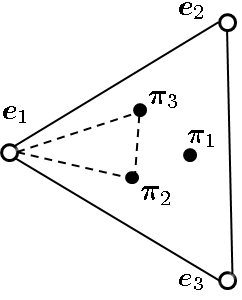
\includegraphics[width=1.5in]{example_fig.png}
\caption{This is a random figure. In this case the source file type is
{\tt .png}, which means you have to compile with {\tt pdflatex}. For {\tt
.eps} files, you can compile with the command {\tt latex}, and then use
{\tt dvipdfm} to convert to {\tt .pdf}.} \label{fig:example} \end{figure}

\section{Interesting Result}

Your section titles should be tailored to the topic.

\begin{thm}
For any discrimination rule and any sample size, there exists a
distribution such that the risk of the learned classifier is arbitrarily
close to one half, with high probability (paraphrase).
\end{thm}
\begin{proof}
The proof may be found in \cite{devroye96,devroye82}.
\end{proof}
By this result, there is no such thing as a universal rate of
convergence. Any rate of convergence theorem must make some assumption
about the distribution.

\section*{Exercises} % * makes this an unnumbered section

\begin{enumerate}
\item In this problem you will examine rates
of convergence.
\begin{itemize}
\item[(a)] Show that the learning rule described in Section 2 converges at
a rate of $n^{-\alpha}$.
\item[(b)] Show that this is the fastest possible rate of any learning
algorithm.
\end{itemize}
\end{enumerate}

%%
%% Bibliography -- For simplicity please hardcode the bibliography entries
%% as illustrated below, rather than using bibtex.
%%
%% If you paste the bibliography entry from a bibtex file, you may need to
%% edit the paper information somewhat to conform to the style set forth
%% in this template.
%%

\begin{thebibliography}{10}
\bibitem{devroye96}
L. Devroye, L. Gy{\"o}rfi and G. Lugosi,
{\it A Probabilistic Theory of Pattern Recognition}, Springer, 1996.
\bibitem{devroye82}
L. Devroye, ``Any discrimination rule can have an arbitrarily bad
probability of error for finite sample size," {\it IEEE Trans. Pattern
Analysis and Machine Intelligence}, vol. 4, pp. 154-157, 1982.
\end{thebibliography}

\end{document}




